\documentclass[11pt]{article}
\usepackage[final]{acl}
\usepackage{times}
\usepackage{latexsym}
\usepackage[T1]{fontenc}
\usepackage[utf8]{inputenc}
\usepackage{microtype}
\usepackage{inconsolata}
\usepackage{booktabs}
\usepackage{amsmath}
\usepackage{amssymb}
\usepackage{multirow}
\usepackage{xcolor}
\usepackage{graphicx}

\title{Say It as a Premise, Not a Shortlist:\\A Form-Dependent Keep--Rescue Trade-off in Team-Wide Notes to LLM Nodes}

\author{Shilin Yin \\
  University of Westminster \\
  \texttt{syin31437@gmail.com}}

\begin{document}
\maketitle

\begin{abstract}
A note broadcast to a whole team of language-model ``nodes'' reaches nodes that answered correctly and nodes that answered wrongly, and the sender knows neither which is which nor whether the note is true. We ask which \emph{form} of such a blind broadcast best trades rescuing the wrong nodes against keeping the right ones. For the same question we write a true and a false note in each form, give each to every node after it has answered once, and measure the keep rate $K$ of nodes that were right and the rescue rate $B$ of nodes that were wrong; the two combine into $v^\ast$, the smallest probability that the note is true at which broadcasting it has non-negative expected value. Across eight pre-registered rounds, six to eight nodes per round and ten models in all, on an 80-item and a 297-item set of multiple-choice questions, 80 open-ended rewrites and 51 reading-comprehension items, we find: (i) a false \emph{shortlist} of candidate answers is far more destructive than a false \emph{premise} about the same item ($K$ 29\% vs.\ 86\%); (ii) an exit clause on the shortlist recovers most of the lost keep in every setting at a small rescue cost, but does nothing for premises; (iii) by $v^\ast$ the premise is cheaper than either shortlist form, a margin that holds on every node once the echo of the node's earlier answer is removed and replicates on one of two new model families (the other is not moved by premises at all); (iv) the premise is not cheaper than simply asserting one answer: it keeps far more right nodes ($+.58$) and rescues far fewer wrong ones ($-.63$), with no detectable difference in $v^\ast$; a premise that also names the answer splits the gap, attributing $+.15$ of the premise's safety to its reason and $+.43$ to its not naming an option; (v) with the source passage available, nodes that abandon a correct answer under a false shortlist justify the switch with a genuine quotation 94\% of the time, consistent with picking first and justifying after. Throughout we report $v^\ast$ under a clipped and an unclipped definition and show which conclusions depend on that choice, on a single node, or on the strength of the note. What we observe is a form-dependent trade-off between keeping right nodes and rescuing wrong ones; the data do not establish that nodes check premises. We release items, notes, raw responses and the pre-registrations.
\end{abstract}

\section{Introduction}

Multi-agent systems built from large language models (LLMs) increasingly share information by broadcast: a coordinator posts a hint, a memory, a retrieved fact or a shortlist of candidate answers to every worker \citep{du2024debate}. The broadcast is \emph{blind} in two senses: the sender does not know which workers are currently right, nor whether the note itself is true. A useful note must therefore satisfy two requirements at once: when it is true it should move the workers that were wrong, and when it is false it should not move the workers that were right.

These two requirements are usually studied separately: work on sycophancy and misleading context measures how easily an LLM abandons a correct answer under pressure \citep{sharma2024sycophancy,wang2023defend,xu2024earth}; work on hints and advice measures how much a wrong model benefits from help \citep{bailey2023advice}. Neither asks the broadcaster's question: given that I must send the \emph{same sentence} to everyone, and may be wrong, which form should I send?

We answer this with a paired design. For each item we write a \emph{true} and a \emph{false} version of the note in every form under test; the false version points at a specific wrong option. Every node answers each item once without a note, then again with each note. On the items a node got right we measure the \textbf{keep rate} $K$ (fraction that stay right); on the items it got wrong we measure the \textbf{rescue rate} $B$ (fraction that become right). Combining the true-note and false-note effects with the node's own error rate yields $v^\ast$, the break-even truth probability of the note: a form with lower $v^\ast$ is safer to broadcast.

We compare four forms that differ in what they assert. A \emph{shortlist} names two candidate options (``the correct answer is one of: B, D.''). A \emph{premise} states one key fact or step from which the answer follows, without naming an option. Each may carry an \emph{exit clause} (``\ldots, unless you have strong reasons for another option''; Table~\ref{tab:forms}). A control round adds a bare \emph{assertion} of one option (``the correct answer is B.'') as a strength baseline.

Our contributions are:
\begin{itemize}\itemsep0pt
\item A same-item paired true/false design and the break-even measure $v^\ast$ that turn ``helps the wrong without hurting the right'' into a single pre-registrable number, with its boundary cases and a leave-one-node-out check made explicit (\S\ref{sec:measures}, Appendix~\ref{app:vstar}).
\item Evidence that a false shortlist is the most destructive form (keep 29\% on the 80-item set, 20\% on its hard half), that a false premise about the same item costs far less (86\%, 80\% on the hard half), and that the gap is specific to the shortlist form rather than to multiple-choice formatting (\S\ref{sec:set-vs-premise}).
\item A pre-registered test, replicated on the 80-item set, its 80 open-ended rewrites and 297 fresh items, showing that an exit clause on a shortlist recovers most of the lost keep at a small rescue cost, while the same clause on a premise gives no gain (\S\ref{sec:exit}).
\item A head-to-head by $v^\ast$ (\S\ref{sec:head}) and three pre-registered controls (\S\ref{sec:controls}): the premise is cheaper than both shortlist forms, with a margin over shortlist-with-exit that depends on a definitional choice when the node's earlier answer is echoed and holds on every node when it is not; against a bare single-option assertion the premise is far safer when false and far weaker when true, with no difference in $v^\ast$; a premise that also names the answer separates the reason's share of that safety ($+.15$ keep) from the share owed to not naming an option ($+.43$); a replication on two further open-weight families reproduces the keep-side results on both and the cost ordering on one.
\item A probe on reading comprehension: giving nodes the passage halves the damage of a false shortlist, yet nodes that still switch away quote a true sentence to support the wrong option, a pattern consistent with picking first and justifying after (\S\ref{sec:evidence}).
\end{itemize}

All rounds were pre-registered before the data were collected (\S\ref{sec:setup}); analyses that were not are labelled exploratory.

\section{Measures}
\label{sec:measures}

Let a node answer an item once (the \emph{first answer}) and then again after seeing a note $p$ (the \emph{second answer}). For node $a$ and note form $p$,
\begin{align*}
K_a(p)&=\Pr(\text{second right}\mid \text{first right}),\\
B_a(p)&=\Pr(\text{second right}\mid \text{first wrong}).
\end{align*}
The blank condition ($p=\varnothing$) gives the baselines $K_a^0$, $B_a^0$; in every round that echoes the node's first answer $K^0\ge 0.98$ for multiple-choice items (82--100\% without the echo, \S\ref{sec:set-vs-premise}).

Every form $p$ comes in a true version $p_t$ and a false version $p_f$ for the same item. Let $\varepsilon_a$ be the node's first-answer error rate. The expected change in accuracy from broadcasting the true version is
\begin{align*}
n_t = \;&\varepsilon_a\,[B_a(p_t)-B_a^0]\\&-(1-\varepsilon_a)\,[K_a^0-K_a(p_t)],
\end{align*}
and $n_f$ is defined likewise with $p_f$. If the sender believes the note is true with probability $v$, the expected gain is $v\,n_t+(1-v)\,n_f$, which is non-negative iff
\[
v\;\ge\;v^\ast = \frac{-n_f}{\,n_t-n_f\,}.
\]
$v^\ast$ is the break-even truth probability: a form with $v^\ast=0.84$ should only be broadcast when the sender is at least 84\% sure it is right. The ratio is a threshold only when $n_f<0<n_t$. When the false version does no net harm ($n_f\ge0$) the note is acceptable at any belief and we clip $v^\ast$ to $0$; when the true version does no net good ($n_t\le0$) it is acceptable at none and we clip to $1$. The unclipped ratio is reported alongside and is undefined in those cases; Appendix~\ref{app:vstar} gives the full case analysis, how often each case occurs in our data, and a leave-one-node-out check of every $v^\ast$ comparison. All statistics are node means; confidence intervals are 95\% percentile intervals from 2{,}000 bootstrap resamples over items, with paired differences computed within node and item.

\section{Setup}\label{sec:setup}

\paragraph{Items.} Multiple-choice items come from MMLU \citep{hendrycks2021mmlu} subsets grouped into three task types, \emph{recall} (e.g.\ global facts, astronomy), \emph{reason} (e.g.\ mathematics, formal logic) and \emph{case} (e.g.\ law, clinical medicine); the subsets are listed in Appendix~\ref{app:prompts}. We exclude items whose options refer to other options (``all of the above'', ``both A and B'') and, for the open-ended rewrites, items that cannot be answered without seeing the options. Reading-comprehension items come from RACE \citep{lai2017race}. Three item sets are used:
\begin{itemize}\itemsep0pt
\item \textbf{80-item set}: 40 \emph{hard} items on which at least one frontier model erred in an earlier screening, and 40 \emph{fresh} items from the same sources with no screening (case 56, recall 24).
\item \textbf{297-item set}: from a pool of 1{,}366 unused items, five inexpensive nodes screened for items that at least one node got wrong (635 candidates); 320 were drawn balanced across the three task types, and 297 survived note generation (case 103, reason 98, recall 96).
\item \textbf{RACE set}: 51 passages with one four-option question each.
\end{itemize}
Table~\ref{tab:rounds} lists the eight pre-registered rounds, in the order they were run, with the sections that report them.

\begin{table}[t]
\centering\scriptsize
\setlength{\tabcolsep}{2.5pt}
\begin{tabular}{@{}llll@{}}
\toprule
Round & Items & Nodes & Tests (\S) \\
\midrule
Wording & 80 MC & 6a & W1--3 (\ref{sec:exit}) \\
Format study & 80 MC, 3 formats & 5 of 6a, 2 Claude & \ref{sec:set-vs-premise} \\
Final form & 80 MC $+$ 80 open & 6a & \ref{sec:exit}, \ref{sec:head} \\
RACE & 51, $\pm$passage & 6a & Q1--2 (\ref{sec:evidence}) \\
Scale & 297 MC & 6b & S1--5 (\ref{sec:exit}, \ref{sec:head}) \\
Control & 297 MC, \textsc{one1}, no echo & 6b & E1--2 (\ref{sec:controls}) \\
Named premise & 297 MC, \textsc{L3n} & 6b & F1--3 (\ref{sec:controls}) \\
Replication & 297 MC & Gemma, Mistral & R1--3 (\ref{sec:controls}) \\
\bottomrule
\end{tabular}
\caption{Pre-registered rounds in run order, each with a blank control. 6a = Kimi, Grok, \textsc{Flash-A}, \textsc{Flash-B}, \textsc{Pro}, \textsc{Codex}; 6b = \textsc{Flash-A}, \textsc{Flash-B}, \textsc{Pro}, \textsc{Codex}, \textsc{Qwen}, \textsc{Llama}. The replication round also re-ran \textsc{Flash-B} twice.}
\label{tab:rounds}
\end{table}

\paragraph{Nodes.} We treat each model configuration as a \emph{node}. The main rounds use six nodes: DeepSeek V4 Flash at temperature 0 with a ``precise assistant'' system prompt (\textsc{Flash-A}), DeepSeek V4 Flash at temperature 1 with an ``answer quickly from memory'' prompt (\textsc{Flash-B}; the only sampled node), DeepSeek V4 Pro at temperature 0 with reasoning disabled (\textsc{Pro}), OpenAI Codex CLI with web search disabled (\textsc{Codex}), and, in the earlier rounds, Kimi K3.1 Pro and Grok 4.7 through their command-line interfaces with tools and web access disabled. The 297-item round was pre-registered with eight nodes: these six plus two open-weight models served locally at temperature 0, Qwen2.5-14B-Instruct (\textsc{Qwen}) and Llama-3.1-8B-Instruct (\textsc{Llama}); Kimi and Grok exhausted their quotas mid-run (7\% and 12\% coverage) and were excluded by the pre-registered coverage check, leaving six. Claude Sonnet and Haiku appear only in the format study and as a second judge. A replication round (\S\ref{sec:controls}) adds two open-weight nodes from families not otherwise represented, Gemma 3 12B (\textsc{Gemma}) and Mistral 7B (\textsc{Mistral}), served the same way. No node has conversational memory between calls.

\paragraph{Protocol.} Items are presented in batches of three to five of the same task type. The first prompt asks for a JSON object per item with an answer letter, a confidence and a one-sentence reason. The second prompt repeats the items, echoes the node's own earlier answer, confidence and reason, and appends to each item ``A note shared with the whole team: \ldots''; all items in a batch carry notes of the same condition. The note is identical for every node. The control round (\S\ref{sec:controls}) also runs a variant of the second prompt without the echo, so that the node sees only the items and the note. For open-ended rewrites the options are removed, the node answers in free text, and a separate DeepSeek V4 Pro judge, blind to node and note, grades the stated conclusion against the reference (Cohen's $\kappa=.83$ and $.88$ against two other models' re-grades; Limitations). Full prompts are in Appendix~\ref{app:prompts}.

\paragraph{Forms.} Table~\ref{tab:forms} lists the eight forms. Four (\textsc{set2}, \textsc{cond2}, \textsc{L3}, \textsc{L3c}) are used in the 297-item round; with true and false versions and the blank control they give nine conditions. \textsc{soft2} and \textsc{set3} appear only in the wording round, \textsc{one1} and \textsc{L3n} only in the control rounds. For each item one wrong option is drawn at random (seeded by item id) as the \emph{target}: the false assertion names it, the false premise leads to it, the false shortlist pairs it with a second random wrong option, and the true shortlist pairs the gold option with it. The target is fixed per item and does not depend on the node's own answer. Premises were written by DeepSeek V4 Pro from the item, its gold option and the target: the true premise is a key step from which a careful reader can derive the answer, the false premise is a plausible step that leads to the target. A program rejects premises that name an option letter, quote the gold (true) or target (false) option text, or are shorter than 20 characters; 23 of 320 items were dropped on this check in the 297-item round. The same premise sentences are used across all nodes and all rounds that share an item.

\begin{table}[t]
\centering\footnotesize
\begin{tabular}{@{}lp{5.6cm}@{}}
\toprule
Form & Note text (false version shown where it differs only in the options named) \\
\midrule
\textsc{one1} & the correct answer is B. \\
\textsc{set2} & the correct answer is one of: B, D. \\
\textsc{soft2} & the correct answer is probably one of: B, D. \\
\textsc{cond2} & the correct answer is one of: B, D, unless you have strong reasons for another option. \\
\textsc{set3} & the correct answer is one of: A, B, D. \\
\textsc{L3} & \emph{[one-sentence premise]} \\
\textsc{L3c} & \emph{[premise]} Rely on this unless you have strong reasons to think otherwise. \\
\textsc{L3n} & \emph{[premise]} So the correct answer is B. \\
\bottomrule
\end{tabular}
\caption{Note forms. Each has a true ($t$) and false ($f$) version for the same item. \textsc{one1} false names the designated wrong target. \textsc{set3} true contains the gold option and two wrong ones; false contains three wrong ones.}
\label{tab:forms}
\end{table}

\paragraph{Pre-registration.} Each round's script, item list, thresholds and decision table were committed to a public repository before the run; the results commit follows. The repository, with those commits, the items, notes, raw responses and analysis code, is at \url{https://github.com/syin31437-collab/ring-arith-toy} (directory \texttt{relation/}). Criteria are of the form ``node-mean difference $\ge\theta$, bootstrap lower bound $>0$, and at least $k$ of $n$ nodes in the same direction''. Exploratory analyses are marked as such.

\section{A false shortlist destroys correct answers; a false premise mostly does not}
\label{sec:set-vs-premise}

\begin{figure*}[!t]
\centering
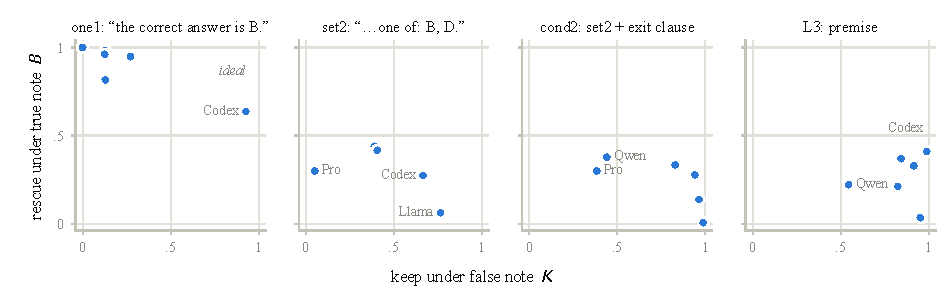
\includegraphics[width=0.52\textwidth]{fig_forms.pdf}
\caption{The trade each form makes: keep under the false note against rescue under the true note, one point per node, 297-item round with echo (\textsc{one1} from the control round, \S\ref{sec:controls}). An assertion moves almost every node; a shortlist loses most right nodes for a modest rescue; the exit clause restores keep on every node but \textsc{Qwen}; a premise keeps right nodes at a cost in rescue.}
\label{fig:forms}
\end{figure*}

Table~\ref{tab:kb} gives node-mean keep and rescue rates for every form in the three multiple-choice rounds. The \emph{true} versions of every form rescue a substantial share of wrong answers (true shortlist 57\% on the 80-item set, true premise 55\%) and keep correct answers almost perfectly. The \emph{false} versions differ sharply: a false shortlist keeps only 29\% of correct answers on the 80-item set (20\% on its 40 hard items) and 45\% on the fresh 297; a false premise about the same item keeps 86\% (80\%) and 85\%. Figure~\ref{fig:forms} plots, per node, keep under the false note against rescue under the true note for the four forms of \S\ref{sec:head}--\S\ref{sec:controls}.

\begin{table*}[t]
\centering\footnotesize
\setlength{\tabcolsep}{4pt}
\begin{tabular}{@{}lcccccc@{}}
\toprule
& \multicolumn{2}{c}{80 items (40 hard)} & \multicolumn{2}{c}{80 items (40 hard)} & \multicolumn{2}{c}{297 fresh items} \\
& \multicolumn{2}{c}{(wording round)} & \multicolumn{2}{c}{(final-form round)} & \multicolumn{2}{c}{(scale round)} \\
Form & $K$ & $B$ & $K$ & $B$ & $K$ & $B$ \\
\midrule
blank & 100 & 0 & 100 & 0 & 100 & 5 \\
\textsc{set2}$_t$ & 99 & 57 & 99 & 57 & 97 & 32 \\
\textsc{set2}$_f$ & \textbf{29} & 0 & \textbf{29} & 0 & \textbf{45} & 3 \\
\textsc{soft2}$_t$ & 99 & 46 & -- & -- & -- & -- \\
\textsc{soft2}$_f$ & 72 & 0 & -- & -- & -- & -- \\
\textsc{cond2}$_t$ & 100 & 42 & 100 & 42 & 98 & 24 \\
\textsc{cond2}$_f$ & \textbf{79} & 0 & \textbf{79} & 0 & \textbf{76} & 5 \\
\textsc{set3}$_t$ & 99 & 21 & -- & -- & -- & -- \\
\textsc{set3}$_f$ & 47 & 0 & -- & -- & -- & -- \\
\textsc{L3}$_t$ & -- & -- & 100 & 55 & 99 & 26 \\
\textsc{L3}$_f$ & -- & -- & \textbf{86} & 5 & \textbf{85} & 7 \\
\textsc{L3c}$_t$ & -- & -- & 99 & 59 & 100 & 32 \\
\textsc{L3c}$_f$ & -- & -- & 83 & 2 & 81 & 7 \\
\bottomrule
\end{tabular}
\caption{Node-mean keep rate $K$ (\% of first-right answers kept) and rescue rate $B$ (\% of first-wrong answers corrected) by form. The two 80-item rounds share items, first answers and nodes (Kimi, Grok, \textsc{Flash-A}, \textsc{Flash-B}, \textsc{Pro}, \textsc{Codex}); the scale round replaces Kimi and Grok with \textsc{Qwen} and \textsc{Llama}.}
\label{tab:kb}
\end{table*}

\paragraph{Is this a multiple-choice artefact?} A pre-registered format study on the 80-item set with seven nodes (Table~\ref{tab:rounds}) presented each item in three conditions: the original batched multiple-choice format (J), single items with options and a three-sentence free-text answer (M), and the same prompt with the options removed (O). In M and O the false shortlist named the option \emph{texts}. Removing the options reduced the damage of the false shortlist only insignificantly ($+.09$ [$-.02$, $+.20$], 3/7 nodes positive), and the batched-JSON format added only $+.08$ [$-.02$, $+.17$]. The pre-registered \emph{form-specificity} test (is the J$-$O difference larger for the shortlist than for the premise?) passed ($+.24$ [$+.11$, $+.37$]): the shortlist loses $.21$ more keep in the batched format while the premise loses nothing ($-.02$). The destructiveness of a false shortlist is thus a property of the form, modulated but not created by the answer format.

\paragraph{Without the echo.} The main rounds echo the node's first answer in the second prompt, so every effect above is measured against a self-anchored prior. A pre-registered control (\S\ref{sec:controls}) re-ran \textsc{blank}, \textsc{set2}, \textsc{cond2} and \textsc{L3} on the 297 items with the echo removed: blank keep falls to 82--100\% and blank rescue rises to 4--26\%, and the premise still keeps more than the shortlist on every node, $K(\textsc{L3}_f)-K(\textsc{set2}_f)=+.19$ [$+.15$, $+.23$], passing the pre-registered keep criterion (difference $\ge.15$, lower bound $>0$, at least four nodes positive; criterion E2c of that round), about half the echoed margin of $+.40$ in Table~\ref{tab:kb}.

Exploratory: on the 80-item set every right node that abandoned its answer under a false shortlist moved \emph{into} the shortlist, never to the unlisted wrong option.

\section{An exit clause rescues the shortlist, not the premise}
\label{sec:exit}

\subsection{Wording round (80 items, 6 nodes)}
The wording round pre-registered three criteria for the exit clause: W1 keep gain $K(\textsc{cond2}_f)-K(\textsc{set2}_f)\ge .15$ with lower bound $>0$ and $\ge 4/6$ nodes positive; W2 rescue cost $B(\textsc{cond2}_t)-B(\textsc{set2}_t)\ge -.15$ with upper bound $<0$ not required; W3 $v^\ast(\textsc{cond2})-v^\ast(\textsc{set2})\le -.10$ with upper bound $<0$. All three passed (Table~\ref{tab:exit}): the clause recovers two-thirds of the lost keep ($+.50$ of $.71$, every node), costs $.14$ rescue, and lowers the break-even truth probability from $.84$ to $.60$. The rescue cost sits on the threshold: in the pre-registered check that drops the two CLI nodes (Grok, \textsc{Codex}) it is $-.19$.

Two alternatives were run in the same round. Hedging (``probably one of'', \textsc{soft2}) behaves like the exit clause ($+.44$ keep, $-.11$ rescue, $v^\ast$ $.84\to.64$). Widening the shortlist to three options (\textsc{set3}) is worse than the exit on both sides: it recovers only $+.18$ keep and loses $.35$ rescue, raising $v^\ast$ to $.91$.

\begin{table*}[t]
\centering\footnotesize
\begin{tabular}{@{}llccc@{}}
\toprule
Round & Criterion & Estimate [95\% CI] & Nodes & Result \\
\midrule
\multirow{3}{*}{80, MC} & keep gain $K(\textsc{cond2}_f)-K(\textsc{set2}_f)$ & $+.50$ [$+.46$, $+.55$] & 6/6 $>0$ & pass \\
& rescue cost $B(\textsc{cond2}_t)-B(\textsc{set2}_t)$ & $-.14$ [$-.23$, $-.05$] & 6 & pass (threshold $-.15$) \\
& $v^\ast(\textsc{cond2})-v^\ast(\textsc{set2})$ & $-.24$ [$-.33$, $-.16$] & 6 & pass \\
\midrule
\multirow{3}{*}{80, open-ended} & keep gain & $+.23$ [$+.18$, $+.29$] & 6/6 $>0$ & pass \\
& rescue cost & $-.03$ [$-.06$, $-.00$] & 6 & pass \\
& $v^\ast$ difference & $-.16$ [$-.20$, $-.11$] & 6 & pass \\
\midrule
\multirow{3}{*}{297 fresh, MC} & keep gain & $+.31$ [$+.28$, $+.34$] & 6/6 $>0$ & pass \\
& rescue cost & $-.08$ [$-.11$, $-.05$] & 6 & pass \\
& $v^\ast$ difference & $-.12$ [$-.25$, $-.01$] & 6 & pass \\
\midrule
\multirow{2}{*}{80, MC (final form)} & exit on premise, keep $K(\textsc{L3c}_f)-K(\textsc{L3}_f)$ & $-.03$ [$-.06$, $+.00$] & 2/6 $>0$ & fail \\
& exit on premise, rescue $B(\textsc{L3c}_t)-B(\textsc{L3}_t)$ & $+.05$ [$+.00$, $+.09$] & 6 & no net gain \\
\multirow{2}{*}{297 fresh, MC} & exit on premise, keep & $-.03$ [$-.05$, $-.01$] & 2/6 $>0$ & fail \\
& exit on premise, rescue & $+.06$ [$+.03$, $+.09$] & 6 & no net gain \\
\bottomrule
\end{tabular}
\caption{Pre-registered tests of the exit clause. Keep gain is measured on false notes, rescue cost on true notes; all differences are paired within node and item. ``Nodes'' gives how many of the available nodes had the difference in the reported direction (keep) or the number of nodes with at least 8 (15 in the scale round) first-wrong items (rescue).}
\label{tab:exit}
\end{table*}

\subsection{Replications}
The exit result replicated twice with the criteria fixed in advance (Table~\ref{tab:exit}): on the 80 items rewritten as open-ended questions (no options; the note names option texts) and on the 297 fresh items, the keep gain is positive on every node and the rescue cost small. Without the echo (\S\ref{sec:controls}) the gain is $+.15$ [$+.13$, $+.18$], 6/6 nodes, on the same threshold (criterion E2b), at a rescue cost of $.05$. The gain is smaller on the small open-weight models (\textsc{Qwen} $+.03$, \textsc{Llama} $+.22$) than on the API nodes ($+.30$ to $+.52$).

\subsection{The clause does nothing for premises}
The final-form round added the exit clause to premises (\textsc{L3c}). On both the 80-item and the 297-item sets the clause slightly \emph{increases} the damage of a false premise ($-.03$ keep, lower bound below zero in the larger set) and slightly increases the rescue of a true premise ($+.05$, $+.06$). The two cancel: $v^\ast(\textsc{L3c})-v^\ast(\textsc{L3})$ is $-.03$ [$-.09$, $+.04$] (unclipped, four defined nodes) and $-.03$ [$-.11$, $+.03$] (clipped, six nodes). The exit clause works by licensing the node to step outside a shortlist; a premise has no inside to step out of.

\section{Premise versus shortlist-with-exit}
\label{sec:head}

\paragraph{Two definitions of $v^\ast$.} The ratio is undefined when $n_f\ge0$ or $n_t\le0$ (Appendix~\ref{app:vstar}). In the 80-item final-form round this happened for Grok and \textsc{Codex} under the false premise, so the pre-registered comparison ran on four nodes; for the 297-item round we therefore pre-registered the clipped definition and committed to report the unclipped version alongside.

\begin{table}[t]
\centering\footnotesize
\setlength{\tabcolsep}{3.5pt}
\begin{tabular}{@{}lcccc@{}}
\toprule
Round & \textsc{set2} & \textsc{cond2} & \textsc{L3} & \textsc{L3c} \\
\midrule
\multicolumn{5}{@{}l}{\emph{clipped definition}} \\
80 items, 6 nodes & .84 & .60 & .38 & .42 \\
297 fresh, 6 nodes & .84 & .71 & .54 & .51 \\
\quad API nodes only (4) & .92 & .78 & .55 & .59 \\
\quad open-weight only (2) & .66 & .58 & .52 & .37 \\
\quad case items & .85 & .75 & .47 & .46 \\
\quad reason items & .80 & .57 & .39 & .50 \\
\quad recall items & .86 & .64 & .58 & .55 \\
\midrule
\quad no echo (\S\ref{sec:controls}) & .75 & .68 & .50 & -- \\
\midrule
\multicolumn{5}{@{}l}{\emph{unclipped definition (defined nodes only)}} \\
80 items & .84 & .60 & .57 (4) & .42 \\
297 fresh & .84 & .71 & .65 (5) & .51 (6) \\
\quad no echo & .75 & .68 & .50 & -- \\
\bottomrule
\end{tabular}
\caption{Break-even truth probability $v^\ast$ (node means). Lower is cheaper to broadcast. Under the unclipped definition the number of nodes with a defined value is given in parentheses when it is fewer than six. The clipped 80-item row was computed after the fact with the definition pre-registered for the 297-item round. The no-echo rows come from the control round, which did not run \textsc{L3c}; with echo, the bare assertion \textsc{one1} scores $.62$ and the named premise \textsc{L3n} $.53$ under both definitions, all six nodes defined.}
\label{tab:vstar}
\end{table}

\paragraph{Results.} Table~\ref{tab:vstar} gives $v^\ast$ for the four main forms. Under either definition and in every round, the plain shortlist is the most expensive of the four and the shortlist with exit is next; the premise, with or without exit, is cheaper on average, and the two premise forms are not distinguishable from each other (\S\ref{sec:exit}). The pre-registered head-to-head comparisons are:

\begin{itemize}\itemsep0pt
\item \textbf{80 items, unclipped (pre-registered).} $v^\ast(\textsc{L3c})-v^\ast(\textsc{cond2})=-.18$ [$-.28$, $-.02$], all 6 nodes defined: pass. $v^\ast(\textsc{L3})-v^\ast(\textsc{cond2})=-.11$ [$-.24$, $+.03$] on the four defined nodes: fail. Clipped, after the fact, 6 nodes: $-.18$ [$-.31$, $-.05$] and $-.22$ [$-.34$, $-.09$] respectively.
\item \textbf{297 fresh, clipped (pre-registered).} $v^\ast(\textsc{L3})-v^\ast(\textsc{cond2})=-.17$ [$-.29$, $-.01$], 6 nodes: pass. Unclipped: $-.06$ [$-.12$, $+.02$] on the five defined nodes (\textsc{Codex} undefined): would fail. $v^\ast(\textsc{L3c})-v^\ast(\textsc{cond2})=-.20$ [$-.32$, $-.06$], 6 nodes, under both definitions.
\end{itemize}

The pass therefore hinges on how a node that a false premise cannot harm is counted: on the 297-item set the false premise left \textsc{Codex} 99\% of its correct answers, the clipped definition scores that as $v^\ast=0$ against $.75$ for shortlist-with-exit, and that one node carries the mean. On the other nodes the two forms are close (\textsc{Llama} $.40$ vs.\ $.50$, \textsc{Pro} $.78$ vs.\ $.90$, \textsc{Flash-B} $.78$ vs.\ $.84$, \textsc{Flash-A} $.65$ vs.\ $.64$, \textsc{Qwen} tied; Table~\ref{tab:pernodev}). Dropping \textsc{Codex} leaves $-.06$ [$-.20$, $+.11$] clipped, while dropping any other node leaves $-.18$ to $-.21$; and without the echo (\S\ref{sec:controls}) the margin is $-.18$ under both definitions ([$-.24$, $-.11$] clipped, [$-.23$, $-.07$] unclipped), holds on every one of the six nodes (Table~\ref{tab:pernodev}) and survives dropping any one of them (Appendix~\ref{app:vstar}).

Neither component is decisive on its own: relative to shortlist-with-exit, the false premise is kept slightly better ($+.08$ and $+.09$ keep, 4/6 nodes positive) and the true premise rescues about as well ($+.12$ [$-.09$, $+.33$] and $+.02$ [$-.03$, $+.08$]).

\section{Pre-registered controls and a replication}
\label{sec:controls}

A control round on the 297-item set and the same six nodes tested two weaknesses of the rounds above: form is confounded with strength, and the echo of the node's first answer (\S\ref{sec:set-vs-premise}). The round added a seventh form, \textsc{one1} (``the correct answer is B.''), and re-ran \textsc{blank}, \textsc{set2}, \textsc{cond2} and \textsc{L3} with the echo removed from the second prompt. Pre-registered criteria: E1b, the premise is \emph{safer} than the bare assertion (keep difference $\ge.15$, lower bound $>0$, at least four nodes positive); E1c, it is \emph{cheaper} (upper bound of the $v^\ast$ difference below zero); E2b and E2c, the exit and premise keep gains pass the same keep criterion without the echo. Passing E1b but failing E1c was to be read as ``safer when false, not cheaper''. A further round added \textsc{L3n}, the premise followed by the assertion (``\ldots\ So the correct answer is B.''), and tested under the E1b criterion F1, $K(\textsc{L3n}_f)-K(\textsc{one1}_f)$, and F2, $K(\textsc{L3}_f)-K(\textsc{L3n}_f)$, with the decision fixed for all four outcomes.

\paragraph{A bare assertion is stronger in both directions.} True, the single-option assertion rescues 64--100\% of wrong nodes ($B(\textsc{one1}_t)-B(\textsc{set2}_t)=+.57$ [$+.52$, $+.62$]); false, it destroys 73--100\% of correct answers on five nodes, \textsc{Codex} being the exception at 93\%. The two-option shortlist does somewhat less damage when false ($K(\textsc{one1}_f)-K(\textsc{set2}_f)=-.18$ [$-.21$, $-.16$]) but rescues far less when true, and by $v^\ast$ it is the worse deal ($v^\ast(\textsc{set2})-v^\ast(\textsc{one1})=+.21$ [$+.18$, $+.25$], clipped). Shortlist-with-exit is not distinguishable from the bare assertion ($+.09$ [$-.03$, $+.21$]).

\paragraph{The premise is safer than a bare assertion, not cheaper.} E1b passes: $K(\textsc{L3}_f)-K(\textsc{one1}_f)=+.58$ [$+.55$, $+.61$], all six nodes positive (\textsc{Codex} $+.06$). But the true premise rescues far less than the true assertion, $B(\textsc{L3}_t)-B(\textsc{one1}_t)=-.63$ [$-.67$, $-.59$], and the two effects cancel in the break-even probability: $v^\ast(\textsc{L3})-v^\ast(\textsc{one1})=-.08$ [$-.14$, $+.01$] clipped on six nodes, $+.02$ [$-.05$, $+.09$] unclipped on five. E1c fails, and with it the pre-registered conclusion ``the strength confound cannot explain the premise advantage''. The premise's $v^\ast$ advantage in \S\ref{sec:head} is an advantage over \emph{shortlists}, which rescue poorly for the damage they do, not over naming the answer outright.

\paragraph{The reason blocks some of the damage; naming no option blocks more.} Both criteria pass. F1: $K(\textsc{L3n}_f)-K(\textsc{one1}_f)=+.15$ [$+.13$, $+.18$], 5/6 nodes, on the threshold: the reason buys $+.45$, $+.32$ and $+.15$ keep on the three DeepSeek nodes and nothing on \textsc{Codex} ($+.06$), \textsc{Qwen} ($-.06$) or \textsc{Llama} ($+.01$), which follow the named letter whatever precedes it. F2: $K(\textsc{L3}_f)-K(\textsc{L3n}_f)=+.43$ [$+.40$, $+.46$], 6/6 nodes. By the pre-registered reading, the premise's safety is partly its reason and mostly its naming no option; the strength confound is quantified, not removed. The attached reports favour the named premise over the bare assertion: true, it rescues 55--95\% ($-.07$ [$-.10$, $-.04$] below the assertion, $+.56$ [$+.51$, $+.60$] above the bare premise), and its $v^\ast$ is lower on five of six nodes ($-.09$ [$-.13$, $-.07$] clipped, $-.09$ [$-.12$, $-.03$] unclipped) and indistinguishable from the bare premise's ($-.01$ [$-.10$, $+.05$]).

\paragraph{Replication on two new model families.} A final round ran the nine main conditions, \textsc{one1} and \textsc{L3n} on Gemma 3 12B and Mistral 7B with fresh first answers (Appendix~\ref{app:pernode}), with per-node criteria fixed in advance: R1 $K(\textsc{cond2}_f)>K(\textsc{set2}_f)$, R2 $K(\textsc{L3}_f)>K(\textsc{set2}_f)$, R3 $v^\ast(\textsc{L3})<v^\ast(\textsc{cond2})$. Both nodes pass R1 ($+.06$, $+.36$) and R2 ($+.22$, $+.60$); \textsc{Gemma} passes R3 ($.50$ vs.\ $.66$) and \textsc{Mistral} fails it because premises do nothing to it either way: a false one leaves 99\% of its correct answers and a true one rescues 1\%, the blank rate, so $n_t\le0$ and $v^\ast(\textsc{L3})$ is clipped to 1. By the pre-registered wording this is a partial replication. Pooling all eight nodes (exploratory) leaves every keep-side test intact (exit $+.28$, premise over assertion $+.64$, F2 $+.51$, all 8/8) but weakens both $v^\ast$-level claims: $v^\ast(\textsc{L3})-v^\ast(\textsc{cond2})=-.09$ [$-.30$, $+.02$], and F1 $+.13$ [$+.10$, $+.15$] on 6/8 nodes, below its threshold.

\paragraph{Without the echo, the ordering sharpens.} E2b and E2c pass on all six nodes (\S\ref{sec:set-vs-premise}, \S\ref{sec:exit}), every $v^\ast$ is lower (Table~\ref{tab:vstar}) and the premise's margin over shortlist-with-exit holds under both definitions (\S\ref{sec:head}). The echo itself pushes the forms apart: with it, keep is lower under a false shortlist ($-.09$ [$-.12$, $-.05$]) and higher under a false premise ($+.12$ [$+.09$, $+.15$]), and rescue is lower on every form ($-.11$ to $-.22$): a node reminded of its wrong answer is harder to move.

\section{With the passage in hand: pick first, justify after}
\label{sec:evidence}

If nodes abandon answers they cannot verify, evidence should protect them; we tested this on RACE reading comprehension, where the evidence is a passage. Six nodes answered 51 questions with the passage, then answered again with a note under two conditions that differ in one line: the passage is shown (E) or replaced by ``The passage is not shown this time.'' (R). Replies had to quote verbatim the one sentence of the passage relied on most, or leave it empty.

\paragraph{Evidence helps.} The pre-registered criterion Q1 asks whether the damage of a false shortlist is larger without the passage: $[K^0_R-K_R(\textsc{set2}_f)]-[K^0_E-K_E(\textsc{set2}_f)]=+.39$ [$+.31$, $+.47$], all six nodes positive. The false premise shows the same pattern more strongly ($+.52$ [$+.45$, $+.59$]): without the passage a false claim about its content is believed.

\paragraph{But the nodes that are fooled are not fabricating.} Q2 asked whether rows that abandon the correct answer under a false shortlist quote empty or fabricated evidence more often than rows that keep it. They do not: 94\% of the 140 abandoning rows quote a genuine sentence, against 97\% of the keeping rows ($+.03$ [$-.02$, $+.08$]). The pattern is what one would see if the task became ``choose between B and D, then find a supporting sentence'', which a passage long enough to answer the question usually contains.

\paragraph{Without the passage, a false premise does produce fabrication.} When the passage is withheld and the note is a false premise \emph{about the passage}, nodes that follow it sometimes quote sentences that do not exist: 20\%, 22\% and 65\% of \textsc{Flash-A}, \textsc{Flash-B} and \textsc{Pro} responses contain a quotation not in the text, against 0--2\% (8--12\% on \textsc{Pro}) under shortlist notes. A confident false claim about evidence the node cannot see is both believed and back-filled.

\section{Related work}

\paragraph{Misleading context and sycophancy.} LLMs change correct answers when the prompt supplies a wrong one: all-wrong option sets \citep{goral2025wait}, misleading in-context statements, false \citep{wang2026misleadqa} or true but pointing the wrong way \citep{shafiei2026truthtrap}, user challenges \citep{wang2023defend} and persuasive misinformation \citep{xu2024earth}. Sycophancy \citep{sharma2024sycophancy,wei2023synthetic}, knowledge conflict \citep{xie2024chameleon,xu2024conflicts} and distraction \citep{shi2023distracted} are related failures. These studies measure the false-note side alone, so they cannot say what a form costs a sender who is sometimes right.

\paragraph{Hints, advice and abstention.} Hints improve LLM accuracy depending on their form \citep{marioriyad2025unspoken}; people weight advice at about $.39$ of their own judgement \citep{bailey2023advice}; selective prediction \citep{kamath2020selective} lets a model decline when uncertain, as the exit clause lets a node.

\paragraph{Multi-agent debate.} Agents that see each other's answers can improve factuality \citep{du2024debate}; the same channel propagates manipulated knowledge \citep{ju2024flooding}, and re-answering without new information does not correct reasoning \citep{huang2024selfcorrect}. $v^\ast$, a break-even probability in the sense of decision analysis \citep{howard1966}, bounds how confident a writer should be before posting to all.

\section{Discussion}

\paragraph{What a coordinator should post.} A bare assertion is the strongest note in both directions; a premise moves far fewer nodes either way, at the same break-even probability. When losing a correct answer is worse than missing a rescue, the premise is the form to use: a false premise costs a fifth to a quarter of what a false shortlist or assertion costs, and the true premise's rescue is not distinguishable from shortlist-with-exit's ($+.12$ [$-.09$, $+.33$], $+.02$ [$-.03$, $+.08$]). A coordinator that can only name candidates should name one if it values rescue as much as keep, two with an exit clause if not, and never widen the list; one that can name the answer should give the reason with it. These prescriptions rest on six to eight models, one run per node and about twenty uncorrected tests; on \textsc{Mistral} the premise is inert, and one node's $v^\ast$ margin varies between runs by as much as the effect (Limitations).

\paragraph{Form, not mechanism.} The premise's advantage is a form-dependent trade-off, consistent with nodes checking the reason but not proof of it: a weaker push would look the same, and the reason's share is concentrated on three nodes (\S\ref{sec:controls}).
\section{Limitations}

\paragraph{Scope of items.} Our items are English multiple-choice and short open-ended questions from academic subjects and one reading-comprehension corpus; we do not claim the results for code, planning or long-form generation, where an earlier exploratory round found much higher keep rates. The false notes point at one designated wrong option; adversarially optimised notes could do more damage.

\paragraph{Strength.} A false shortlist excludes two options with certainty, whereas a false premise is a model-written sentence whose persuasiveness we did not calibrate. The bare-assertion control (\S\ref{sec:controls}) does not resolve it: the premise is far safer than the strongest option-format note when false and no cheaper by $v^\ast$, a pattern a weaker push would also produce, and the pre-registered test that would have ruled strength out failed. The named-premise round matches the assertion in strength and attributes $+.15$ of the premise's keep advantage to the reason and $+.43$ to naming no option, but the reason's share is carried by the three DeepSeek nodes and is small or zero on the other five. What we still lack is a premise matched to the \emph{shortlist} in strength, or a length- and specificity-matched pair of premises; the split we report is for one strength anchor and one family of models.

\paragraph{Premise quality.} Premises were written by one model (DeepSeek V4 Pro), which also serves as a node, and were checked programmatically (no option letters, no gold or target option text, minimum length). After the 297-item round the author hand-audited 40 randomly drawn items and 33 flagged items (29 because at least two of three strong nodes gave the same wrong first answer, using only note-free answers, plus the four defective items already found in the random audit), 69 distinct items in all. In the random 40, 36 true premises were true and did not state the answer, and 25 false premises were false and read as plausible wrong reasoning, the other 15 being implausible or vacuous; whether a false premise was plausible made no difference to how often it was followed (node-mean keep 83\% vs.\ 84\%; shortlist 42\% vs.\ 38\%), so the premise's safety is not an artefact of unconvincing false premises. Across both audits ten items were defective: five with a wrong, contested or corrupted answer key or a truncated question, and five with a premise pair that failed in ways the program check does not catch (a premise that states an option, a true premise that points at the target, a false premise that leads to a non-target option). A pre-registered sensitivity analysis drops these ten and recomputes every test of \S\ref{sec:exit}--\S\ref{sec:controls} on the remaining 287 items: every direction and decision is unchanged, and no node-mean difference moves by more than $.02$ (e.g.\ $v^\ast(\textsc{L3})-v^\ast(\textsc{cond2})$ on the 297-item set is $-.17$ [$-.29$, $-.01$] before and $-.16$ [$-.28$, $-.00$] after), with one exception: the unclipped premise-versus-assertion difference moves from $+.02$ on five nodes to $-.09$ [$-.12$, $+.08$] on six, because \textsc{Codex}'s unclipped $v^\ast(\textsc{L3})$ becomes defined (at $0$) once the ten items are dropped; E1c still fails. The random audit was not pre-registered.

\paragraph{Echo.} The main rounds echo the node's earlier answer, confidence and reason in the second prompt, so blank keep is $\approx100\%$ and every effect is measured against a self-anchored prior. The no-echo control (\S\ref{sec:controls}) shows that the orderings survive without it, but the echo lowers rescue on every form, lowers keep under a false shortlist and raises it under a false premise, so the premise's keep margin halves without it; the absolute rates in our tables are specific to the echoed protocol.

\paragraph{Statistics.} Six nodes per main round, eight with the replication, is a small sample of models, and all but \textsc{Flash-B} are deterministic (temperature 0) with one run per item, so within-node sampling variance is not captured by the item bootstrap. \textsc{Flash-B} (temperature 1) was run three times on the second prompt of the 297-item round: per-form $K$ and $B$ have SD $\le.045$ across runs, the exit and premise keep gains range $+.42$ to $+.45$ and $+.42$ to $+.52$, and $v^\ast(\textsc{L3})-v^\ast(\textsc{cond2})$ ranges $-.02$ to $-.19$ without changing sign, so a single node's $v^\ast$ difference is as noisy as the effect itself. Items within a batch of three to five share one prompt and one condition, so they are not fully independent; the bootstrap resamples items, not batches. Rescue denominators are as small as 11 (\textsc{Codex}, 80 items) and 22 (\textsc{Codex}, 297 items). Node means of a clipped ratio are fragile: one node at exactly 0 can decide the ordering, which is why \S\ref{sec:head} reports both definitions and Appendix~\ref{app:vstar} drops each node in turn; a node mean of clipped values mixes thresholds with decisions and is used only to order forms, never as a belief level. Per-node numbers are not stable traits: an attempt to predict which nodes a form would rescue from two fitted coordinates failed to transfer (Appendix~\ref{app:negative}). We report every pre-registered test (about twenty decision criteria across eight rounds) without correcting for multiple comparisons. Two of the eight nodes in the largest round were lost to quota exhaustion and are excluded by a pre-registered coverage check; the pre-registered minimum of five nodes was met. The control rounds reuse the 297 items and the same six nodes, so they replicate the protocol but not the item sample.

\paragraph{Judging.} Open-ended answers were graded by a model (DeepSeek V4 Pro; $\kappa=.83$ against a Codex re-grade of 100 rows, $.88$ against an earlier Claude Sonnet grade); it judges the stated conclusion, not the quality of the reasoning.

\section*{Ethics statement}
All items are from public benchmarks. The false notes were generated for measurement and are released only together with their true counterparts and the gold labels. The findings describe how to write notes that help a team of models; they could also inform someone trying to mislead a model, but the misleading forms we identify (a bare shortlist or a bare assertion) are already the default in many pipelines and the contribution is to show how to make it safer.

\bibliography{custom}

\appendix

\section{Prompts}
\label{app:prompts}

\paragraph{MMLU subsets.} \emph{Recall}: global facts, prehistory, astronomy, miscellaneous, US foreign policy. \emph{Reason}: high-school and college mathematics, statistics, physics, formal logic, abstract algebra, econometrics. \emph{Case}: professional and international law, jurisprudence, clinical knowledge, college and professional medicine.

\paragraph{System prompts.} \textsc{Flash-A} and \textsc{Pro}: \texttt{You are a precise data assistant.} \textsc{Flash-B}: \texttt{Answer quickly from memory; rough estimates are fine.} The CLI and open-weight nodes receive no system prompt beyond the tool-disabling flags described in \S\ref{sec:setup}.

\paragraph{First answer (multiple choice).} ``Answer each question.'' followed by the items, then: \texttt{Reply with ONLY a JSON object mapping each question ID to \{"answer": "A/B/C/D", "confidence": 0-100, "reason": "one short sentence"\}. No prose outside the JSON.}

\paragraph{Second answer.} ``Here are questions you answered earlier. Give your answer again.'' followed, per item, by the item text, \texttt{Your earlier answer: X (confidence N). Your earlier reason: \ldots} and, unless blank, \texttt{A note shared with the whole team: \ldots}; then the same JSON instruction. In the no-echo variant of the control round the \texttt{Your earlier answer} and \texttt{Your earlier reason} lines are omitted and nothing else changes.

\paragraph{Open-ended.} The item without options; \texttt{Here is a task you answered earlier. Give your answer again.} with the earlier free-text answer echoed; the note names option texts (``the correct answer is one of: 36\%; 81\%.''). Judge prompt: \texttt{Grade each response against the reference. Mark correct = 1 only if the response's stated conclusion agrees with the reference; hedging without the right conclusion, or a contradictory answer, is 0. Ignore style and extra detail.}

\paragraph{Premise generation.} Given the question, options, gold option and target wrong option, DeepSeek V4 Pro was asked for a JSON object with \texttt{L3t}: ``the true key premise or step from which a careful reader could work out the answer. Do not state the answer or repeat the correct option text.'' and \texttt{L3f}: a matched misleading premise that leads to the target option, under the same constraints.

\section{The break-even probability: cases, occurrence and node sensitivity}
\label{app:vstar}

\paragraph{Cases.} With $n_t$ and $n_f$ the expected accuracy change from the true and the false version of a note (\S\ref{sec:measures}), the expected gain of broadcasting under belief $v$ is $g(v)=v\,n_t+(1-v)\,n_f$, linear in $v$. Four cases arise.
\begin{itemize}\itemsep0pt
\item[A] $n_f<0<n_t$: $g$ crosses zero once, at $v^\ast=-n_f/(n_t-n_f)\in(0,1)$. This is the only case in which $v^\ast$ is a threshold; the clipped and unclipped definitions agree.
\item[B] $n_f\ge0$ and $n_t\ge0$: $g(v)\ge0$ for every $v$; the note is acceptable at any belief. Clipped $v^\ast=0$; the unclipped ratio is $\le0$ or undefined.
\item[C] $n_f\le0$ and $n_t\le0$ (not both zero): $g(v)\le0$ for every $v$; the note is acceptable at no belief. Clipped $v^\ast=1$; the unclipped ratio is $\ge1$ or undefined.
\item[D] $n_f>0>n_t$: the false version helps and the true one hurts, $g$ is decreasing, and the note is acceptable only when $v\le n_f/(n_f-n_t)$. The formula returns that number, but with its meaning reversed. We clip this case to $0$ with case B; it did not occur.
\end{itemize}
The clipped values $0$ and $1$ encode the sender's decision in cases B and C, not a belief. A node mean over clipped values therefore mixes thresholds with decisions; we use it only to order forms and check every ordering under the unclipped definition on the nodes where it is defined.

\paragraph{Occurrence.} Over the 297-item round and the control rounds with echo (six nodes, six forms: \textsc{set2}, \textsc{cond2}, \textsc{L3}, \textsc{L3c}, \textsc{one1}, \textsc{L3n}) 35 of 36 node--form cells are in case A; the one exception is \textsc{Codex} under \textsc{L3}, with $n_f=.000$ (case B), which is the cell that decides the echoed S1 comparison in \S\ref{sec:head}. Without the echo all 18 cells are in case A. In the replication round 10 of 12 cells are in case A and two are in case C: \textsc{Mistral} under \textsc{L3} and \textsc{L3c}, with $n_t\approx0$ (the premise is inert). Case D did not occur. Some case-A values rest on tiny denominators: \textsc{Llama} under \textsc{cond2} has $n_t=+.003$ and $n_f=-.003$, so its $v^\ast=.50$ reflects a net change of about one item in each direction.

\paragraph{Statistics.} $v^\ast$ is a ratio of two differences of item means. Intervals are 95\% percentile intervals over 2{,}000 item resamples, recomputing each node's $v^\ast$ and the node mean on every resample, so they are intervals for the node mean of per-node values and are only as stable as the per-node denominators. The three Flash-B runs (Limitations, ``Statistics'') put the run-to-run range of a single node's $v^\ast(\textsc{L3})-v^\ast(\textsc{cond2})$ at $.17$, comparable to the effect.

\paragraph{Leave one node out.} Table~\ref{tab:loo} recomputes the three $v^\ast$ comparisons that the paper's conclusions rest on with each node dropped in turn (1{,}000 resamples). The echoed premise-versus-exit margin (S1) loses its lower bound when \textsc{Codex} is dropped ($-.06$ [$-.20$, $+.11$]) and marginally when \textsc{Pro} is dropped ([$-.32$, $+.01$]); the unechoed margin (E2d) keeps a negative upper bound whichever node is dropped, under both definitions; the premise-versus-assertion comparison (E1c) is not resolved in any subset under the unclipped definition and reaches a negative upper bound under the clipped definition only when \textsc{Qwen} or \textsc{Llama} is dropped. This analysis was not pre-registered.

\begin{table*}[h]
\centering\scriptsize
\setlength{\tabcolsep}{2.2pt}
\begin{tabular}{@{}lcccccc@{}}
\toprule
& \multicolumn{2}{c}{S1: $v^\ast(\textsc{L3})-v^\ast(\textsc{cond2})$, echo} & \multicolumn{2}{c}{E2d: same, no echo} & \multicolumn{2}{c}{E1c: $v^\ast(\textsc{L3})-v^\ast(\textsc{one1})$, echo} \\
\cmidrule(lr){2-3}\cmidrule(lr){4-5}\cmidrule(lr){6-7}
Dropped & clipped & unclipped & clipped & unclipped & clipped & unclipped \\
\midrule
none & $-.17$ [$-.29$, $-.01$] (6) & $-.06$ [$-.12$, $+.02$] (5) & $-.18$ [$-.25$, $-.10$] & $-.18$ [$-.23$, $-.07$] & $-.08$ [$-.14$, $+.00$] (6) & $+.02$ [$-.05$, $+.09$] (5) \\
\textsc{Flash-A} & $-.21$ [$-.34$, $-.03$] & $-.07$ [$-.13$, $+.00$] & $-.20$ [$-.28$, $-.13$] & $-.20$ [$-.25$, $-.08$] & $-.07$ [$-.13$, $+.03$] & $+.06$ [$-.01$, $+.14$] \\
\textsc{Flash-B} & $-.19$ [$-.32$, $-.01$] & $-.05$ [$-.12$, $+.04$] & $-.21$ [$-.28$, $-.13$] & $-.21$ [$-.26$, $-.08$] & $-.09$ [$-.15$, $+.01$] & $+.03$ [$-.04$, $+.11$] \\
\textsc{Pro} & $-.18$ [$-.32$, $+.01$] & $-.04$ [$-.11$, $+.06$] & $-.20$ [$-.27$, $-.11$] & $-.20$ [$-.25$, $-.06$] & $-.09$ [$-.15$, $+.00$] & $+.03$ [$-.04$, $+.11$] \\
\textsc{Codex} & $-.06$ [$-.20$, $+.11$] & $-.06$ [$-.12$, $+.02$] & $-.10$ [$-.14$, $-.05$] & $-.10$ [$-.14$, $-.05$] & $+.02$ [$-.06$, $+.09$] & $+.02$ [$-.05$, $+.09$] \\
\textsc{Qwen} & $-.20$ [$-.34$, $-.01$] & $-.07$ [$-.14$, $+.03$] & $-.19$ [$-.26$, $-.11$] & $-.19$ [$-.24$, $-.05$] & $-.13$ [$-.20$, $-.03$] & $-.03$ [$-.11$, $+.06$] \\
\textsc{Llama} & $-.19$ [$-.25$, $-.10$] & $-.04$ [$-.11$, $+.02$] & $-.18$ [$-.25$, $-.09$] & $-.18$ [$-.23$, $-.04$] & $-.12$ [$-.16$, $-.05$] & $-.01$ [$-.06$, $+.05$] \\
\bottomrule
\end{tabular}
\caption{Leave-one-node-out recomputation of the three $v^\ast$ comparisons on the 297-item set (node means, 95\% bootstrap intervals over items). Parentheses in the first row give the number of nodes with a defined value; dropping a node removes one from each count. Under the unclipped definition \textsc{Codex} is undefined for \textsc{L3} with echo, so dropping it changes nothing there. The ``none'' row uses 1{,}000 resamples and can differ from the body's 2{,}000-resample intervals by $.01$.}
\label{tab:loo}
\end{table*}

\begin{table}[h]
\centering\scriptsize
\setlength{\tabcolsep}{3.5pt}
\begin{tabular}{@{}lcccccccc@{}}
\toprule
& \multicolumn{4}{c}{with echo} & \multicolumn{3}{c}{without echo} \\
\cmidrule(lr){2-5}\cmidrule(lr){6-8}
Node & \textsc{set2} & \textsc{cond2} & \textsc{L3} & \textsc{L3c} & \textsc{set2} & \textsc{cond2} & \textsc{L3} \\
\midrule
\textsc{Flash-A} & .90 & .64 & .65 & .58 & .76 & .64 & .58 \\
\textsc{Flash-B} & .91 & .84 & .78 & .75 & .74 & .66 & .63 \\
\textsc{Pro} & .93 & .90 & .78 & .81 & .90 & .83 & .74 \\
\textsc{Codex} & .95 & .75 & .00$^\dagger$ & .20 & .89 & .80 & .23 \\
\textsc{Qwen} & .66 & .65 & .65 & .61 & .60 & .59 & .45 \\
\textsc{Llama} & .67 & .50 & .40 & .13 & .60 & .53 & .34 \\
\midrule
\textsc{Gemma} & .61 & .66 & .50 & .42 & -- & -- & -- \\
\textsc{Mistral} & .54 & .54 & 1.00$^\ddagger$ & 1.00$^\ddagger$ & -- & -- & -- \\
\bottomrule
\end{tabular}
\caption{Per-node clipped $v^\ast$ on the 297-item set. $^\dagger$case B ($n_f=0$, unclipped undefined); $^\ddagger$case C ($n_t\le0$). All other cells are case A, where clipped and unclipped values coincide. Without the echo every node has $v^\ast(\textsc{L3})<v^\ast(\textsc{cond2})$.}
\label{tab:pernodev}
\end{table}

\section{A negative result on node-level parametrisation (exploratory)}
\label{app:negative}

In earlier rounds we tried to summarise each node by two coordinates fitted on calibration items (``takes the form'' and ``distinguishes true from false'') and to predict which nodes a form would rescue. The coordinates predicted the ordering of nodes on held-out hard items but not the absolute rates, and they did not transfer to open-ended tasks or to non-LLM rule-based nodes. We report this to discourage treating the per-node numbers in our tables as stable traits.

\section{Per-node results, 297-item round}
\label{app:pernode}

\begin{table*}[h]
\centering\scriptsize
\setlength{\tabcolsep}{3pt}
\begin{tabular}{@{}lrrcccccccc@{}}
\toprule
Node & right & wrong & \textsc{set2}$_t$ & \textsc{set2}$_f$ & \textsc{cond2}$_t$ & \textsc{cond2}$_f$ & \textsc{L3}$_t$ & \textsc{L3}$_f$ & \textsc{L3c}$_t$ & \textsc{L3c}$_f$ \\
\midrule
\textsc{Flash-A} & 239 & 58 & 100/41 & 42/5 & 100/28 & 94/14 & 100/33 & 92/14 & 100/38 & 92/16 \\
\textsc{Flash-B} & 240 & 57 & 100/44 & 39/9 & 99/33 & 83/12 & 100/37 & 84/12 & 100/40 & 83/18 \\
\textsc{Pro} & 240 & 57 & 100/30 & 5/0 & 100/30 & 38/0 & 100/21 & 82/0 & 100/28 & 72/0 \\
\textsc{Codex} & 275 & 22 & 99/27 & 67/0 & 100/14 & 96/0 & 100/41 & 99/9 & 100/50 & 99/0 \\
\textsc{Qwen} & 143 & 154 & 86/42 & 41/2 & 90/38 & 44/1 & 97/22 & 55/8 & 99/31 & 44/8 \\
\textsc{Llama} & 85 & 212 & 96/6 & 76/0 & 100/0 & 99/0 & 99/3 & 95/0 & 100/3 & 98/0 \\
\midrule
\textsc{Gemma} & 123 & 169 & 98/18 & 65/0 & 100/12 & 71/0 & 100/9 & 87/1 & 100/23 & 78/1 \\
\textsc{Mistral} & 92 & 197 & 96/27 & 39/0 & 100/11 & 75/0 & 99/1 & 99/1 & 99/0 & 99/0 \\
\bottomrule
\end{tabular}
\caption{Per node: number of first-right and first-wrong items, and $K/B$ (\%) per form; the last two rows are the replication nodes (\S\ref{sec:controls}), whose counts cover the items with a parsed first and blank answer (292 and 289 of 297; 296 items are parsed by at least one of the two). \textsc{Llama} is almost never rescued by any note; \textsc{Pro} keeps only 5\% under a false shortlist and 38\% with the exit clause, yet 82\% under a false premise; \textsc{Mistral} is untouched by premises in either direction.}
\end{table*}

\begin{table*}[h]
\centering\scriptsize
\setlength{\tabcolsep}{3pt}
\begin{tabular}{@{}lccccccccccccc@{}}
\toprule
& \multicolumn{4}{c}{with echo} & \multicolumn{7}{c}{without echo} & \multicolumn{2}{c}{$v^\ast$} \\
\cmidrule(lr){2-5}\cmidrule(lr){6-12}\cmidrule(lr){13-14}
Node & \textsc{one1}$_t$ & \textsc{one1}$_f$ & \textsc{L3n}$_t$ & \textsc{L3n}$_f$ & \textsc{blank} & \textsc{set2}$_t$ & \textsc{set2}$_f$ & \textsc{cond2}$_t$ & \textsc{cond2}$_f$ & \textsc{L3}$_t$ & \textsc{L3}$_f$ & \textsc{one1} & \textsc{L3n} \\
\midrule
\textsc{Flash-A} & 100/95 & 27/2 & 100/74 & 72/14 & 97/9 & 98/40 & 72/3 & 98/38 & 84/5 & 100/55 & 79/7 & .79 & .66 \\
\textsc{Flash-B} & 100/98 & 13/5 & 100/86 & 45/7 & 92/26 & 95/53 & 71/7 & 97/41 & 80/9 & 98/53 & 74/18 & .82 & .78 \\
\textsc{Pro} & 100/100 & 0/0 & 100/91 & 15/0 & 100/7 & 98/47 & 38/4 & 98/49 & 60/0 & 99/53 & 71/14 & .81 & .80 \\
\textsc{Codex} & 100/64 & 93/0 & 100/55 & 99/0 & 100/9 & 100/36 & 85/0 & 100/23 & 97/5 & 100/55 & 99/14 & .56 & .19 \\
\textsc{Qwen} & 99/96 & 13/3 & 100/95 & 6/2 & 95/4 & 90/41 & 43/3 & 87/35 & 62/1 & 96/38 & 62/6 & .45 & .48 \\
\textsc{Llama} & 100/82 & 13/0 & 100/91 & 14/0 & 82/9 & 67/39 & 12/3 & 73/39 & 29/2 & 85/37 & 51/8 & .30 & .28 \\
\midrule
\textsc{Gemma} & 100/85 & 23/0 & 100/93 & 17/0 & -- & -- & -- & -- & -- & -- & -- & .40 & .40 \\
\textsc{Mistral} & 100/94 & 2/0 & 100/85 & 16/0 & -- & -- & -- & -- & -- & -- & -- & .33 & .32 \\
\bottomrule
\end{tabular}
\caption{Control rounds (\S\ref{sec:controls}), same items and nodes: $K/B$ (\%) for the bare single-option assertion and the named premise with echo, and for the main forms with the echo removed; the last two columns are the clipped $v^\ast$ of the bare assertion and of the named premise. The replication nodes (last two rows) did not run the no-echo arm. The true assertion rescues almost every wrong node; the false one destroys almost every right one except on \textsc{Codex}. Prefixing the reason to the assertion keeps 45, 32 and 15 more points on the three DeepSeek nodes and changes nothing on the other three.}
\end{table*}

\end{document}
